\chapter{Background and Related Work} % (fold)
\label{chap:Background and Work}


\section{Multicast Protocols} % (fold)
\label{sec:Mutlicast Protocols}
Multicast communication refers to the simultaneous delivery of data towards an
    arbitrary number of destinations
    \cite{mc_routing_multimedia, mc_comm_multicomputer}.
Numerous network protocols have been developed to facilitate multicast
communication, encompassing both Network Layer as well as Application Layer
    implementations \cite{universal_mc, overlay_mc_routing}.
This chapter first distinguishes Multicast from other communication schemes.
Subsequently, various multicast protocols are introduced.

According to the OSI model \cite{osi1980} Layer 3, known as the Network Layer,
    is responsible for end-to-end delivery of data between nodes.
In computer networks data is transferred through \glspl{pdu}, composed of
    protocol specific control information (e.g. source and destination
    address), along with a payload carrying the actual data.
To establish a path from the sender to the destination(s), packets (Layer 3
    \glspl{pdu}) may traverse multiple intermediate nodes \cite{rfc791_ip}.
This process is called routing and can be classified into various schemes.
For the purpose of this thesis, our primary focus lies on the schemes depicted
    in \autoref{fig:multicast}.
\textit{Unicast} denotes a one-to-one association between a sender and a single
    destination.
\textit{Broadcast} disseminates packets to all nodes within the sender's
    broadcast domain (Layer 2) \cite{broadcast}.
Typically, IP Routers (Layer 3) serve as the boundary of a broadcast domain.
\textit{Multicast} transmits packets to a group of destinations, accommodating
    both one-to-many and many-to-many communication \cite{rfc1112_ip4mc}.
In contrast to Broadcast, Multicast does not necessarily deliver packets to all
    available nodes.
Furthermore, Multicast packets can be delivered beyond the sender's broadcast 
    domain, implying subsequent replication of the packets.

% This layer is responsible for end-to-end delivery of data between nodes across
%     interconnected networks.
% A network comprises interconnected nodes, each assigned a unique address within
%     this network \cite{rfc791_ip}. 
% Data delivery is achieved through the transmission of network packets,
%     consisting of a header containing the source and destination address, along
%     with a payload carrying the actual data.
% If the data size exceeds the maximum transfer unit of Layer 2, it is fragmented
%     into multiple packets and subsequently reassembled.

\begin{figure}[h]
    \begin{center}
        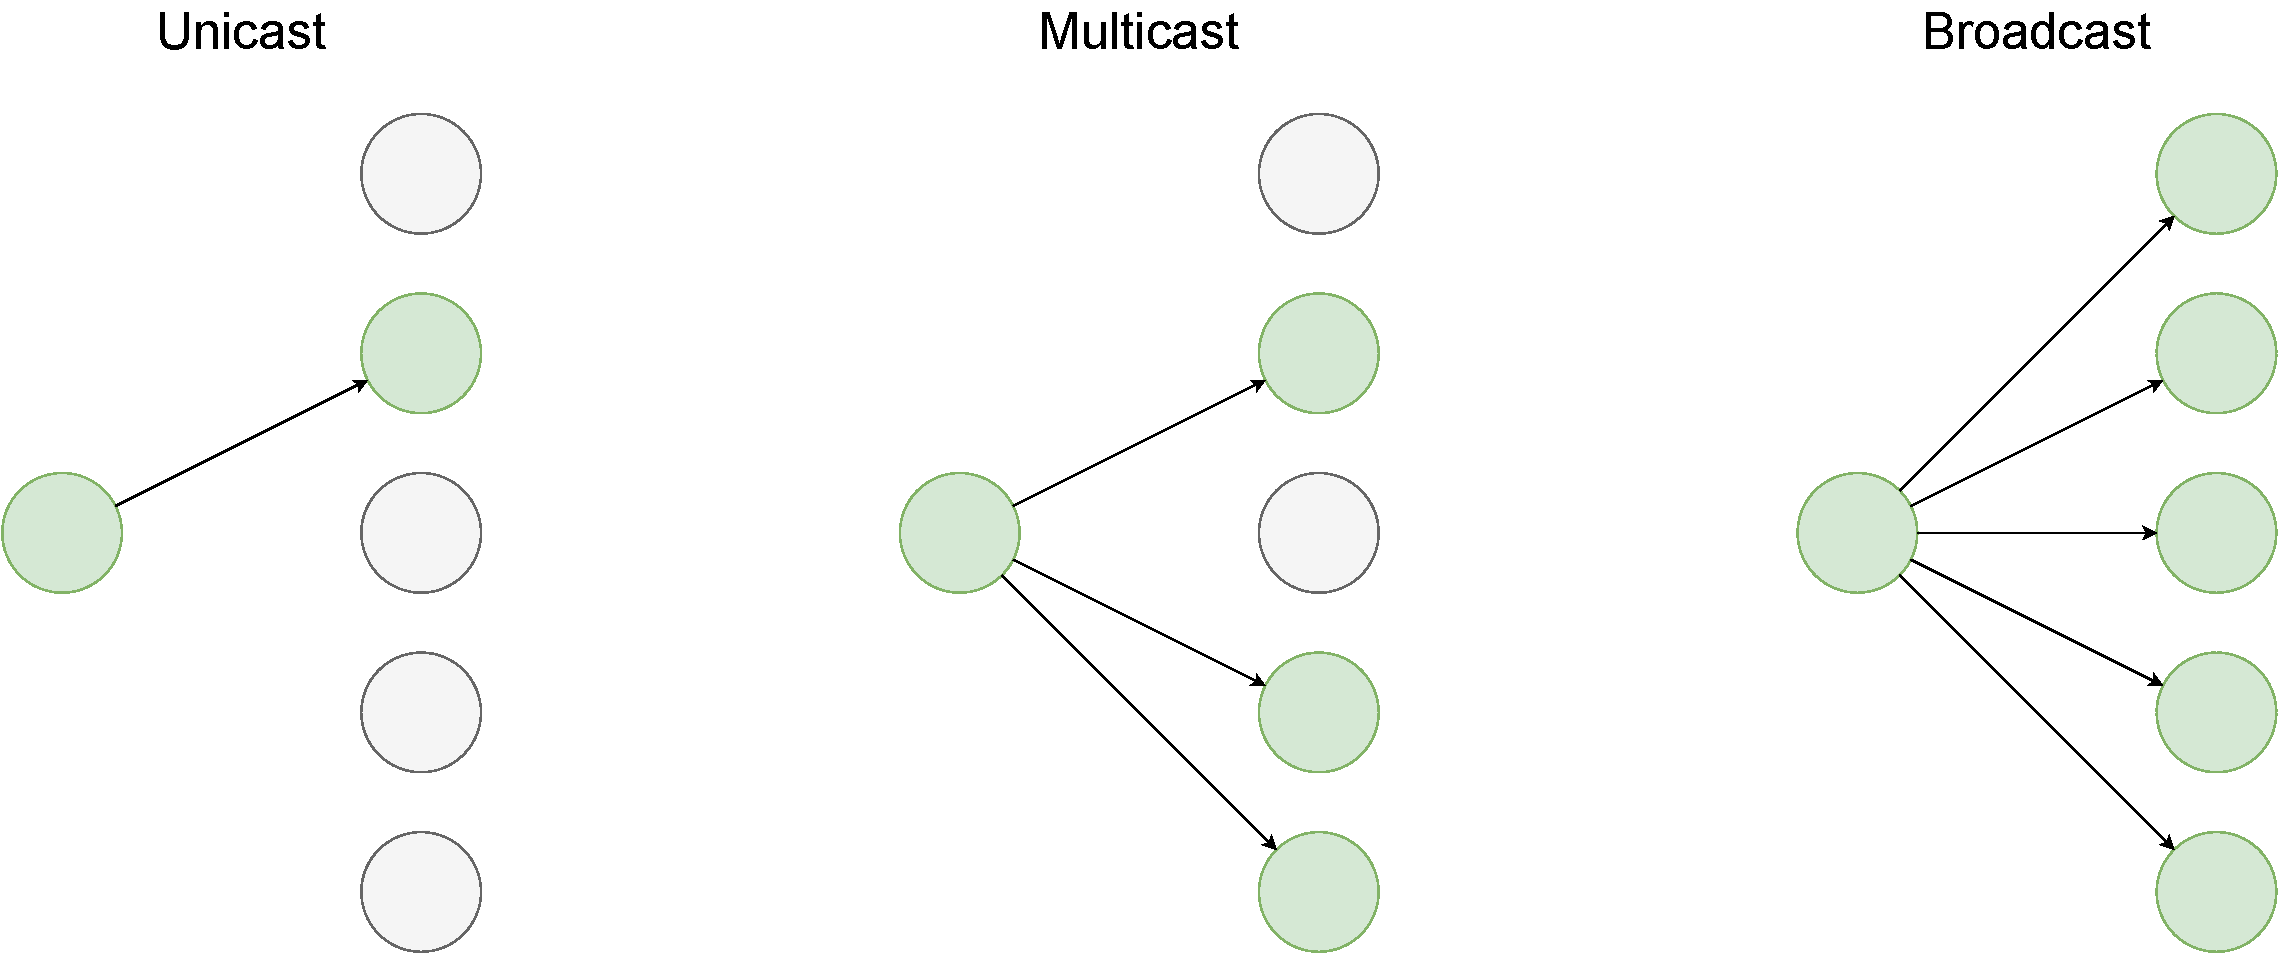
\includegraphics[width=0.85\textwidth]{multicast.pdf}
    \end{center}
    \caption{Network Layer: Routing schemes}
    \label{fig:multicast}
\end{figure}


\subsection{IP Multicast} % (fold)
\label{sub:IP Multicast}
Already in the late 1980s, \citeauthor{deering1990multicast}
    \cite{deering1990multicast} proposed an extension to the IP protocol, to
    facilitate efficient multipoint communication (\textit{1:n}, \textit{m:n}).
This extension is known as IP-Multicast and was first standardized in RFC 988
    (\citeyear{rfc988_initmc}) \cite{rfc988_initmc}.
IP-Multicast offers the advantage, to greatly reduce the bandwidth by condensing
    identical traffic into a single stream targeted to a so called ``Host
    Group'' \cite{rfc1112_ip4mc}.
IP-Multicast operates on a separate address space and host groups are
    identified based on an IP address within the designated address range.
For instance, IPv4 host groups are identified by class D IP addresses starting
    with ``\texttt{1110}'' as their \glspl{msb} \cite{rfc1112_ip4mc}.
This characteristic facilitates high scalability, such that host groups may
    encompass thousands of receivers, since senders are not required of any
    knowledge about the number of receivers nor receivers identity or location.
Intermediate nodes like IP routers replicate multicast packets addressed to an
    host group where the paths towards the receivers diverge.
\begin{itemize}\itemsep0em
    \item Separate address space
    \item IGMP / MLD
    \item Intra-Domain Routing: DVMRP, MOSPF, PIM dense/spare
    \item Inter-Domain Routing: MBGP, MSDP
\end{itemize}
% subsection IP Multicast (end)


% \subsection{Multicast over Unicast} % (fold)
% \label{sub:Multicast over Unicast}
% \begin{itemize}\itemsep0em
%     \item Xcast family (Xcast, Xcast+, GXcast, Xcast6 Treemap (island))
%     \item MEADcast
%     \item Bier
% \end{itemize}

\subsection{Xcast}
\label{sub:Xcast}
Traditional multicast scales well with large multicast groups but has issues
with a high number of distinct groups.
Xcast is a mutlicast protocol with complementary scaling properties compared to
the traditional approach \cite{xcast_rfc}.
The protocol is designed with the key idea of supporting huge numbers of small
multicast sessions.
Xcast achieves this by explicitly encoding the receiver addresses in each
packet, instead of using a multicast addresses \cite{xcast_rfc}.

%%%%%%%%% XCast %%%%%%%%%
% many small groups
% no multicast ips --> no multicast routing
% no per-session signaling and state
% routers must be Xcast capabale or tunneling
% along each path must be an Xcast capabale node (may receiver)

% hdr
% ip
% src: sender
% dst: all_xcast_addr (multicast addrs routers must join)
% xcast
% dsts list of addrs
% protocol id of next header
% bitmap that indicates which addresses needs to be processed
% optional list of ports

%%%%%%%%% XCast+ %%%%%%%%%
% incorporates host group model and Xcast
% enhances routing efficiency
% each sender/receiver has a designated router
% to join a multicast group a receiver sends an IGMP. The DRs intercepts the
% message and sends an registration request msg to the sender. At the senders
% side this msg is intercepted by its DR
% S <--MC--> DR <--XC--> DR <--MC--> R
% Only diff to Xcast is, that the Receivers DRs addresses are encoded in Xcast
% dsts field
% --> better than Xcast, if multiple receivers per DR
% --> DRs keep track, which clients joined the Xcast group (usally via MC)

%%%%%%%%% GXCast %%%%%%%%%
% subsection Xcast (end)

\subsection{MEADcast} % (fold)
\label{sub:MEADcast}

% subsection MEADcast (end)
% section Mutlicast (end)

\section{Linux Kernel} % (fold)
\label{sec:Linux Kernel}

\subsection{Fundamentals} % (fold)
\label{sub:Fundamentals}

% subsection Fundamentals (end)

\subsection{Network Stack} % (fold)
\label{sub:Network Stack}

% subsection Network Stack (end)
% section Linux Kernel Network Internals (end)

% chapter Background Work (end)
